%%
%% This is file `sample-sigplan.tex',
%% generated with the docstrip utility.
%%
%% The original source files were:
%%
%% samples.dtx  (with options: `sigplan')
%% 
%% IMPORTANT NOTICE:
%% 
%% For the copyright see the source file.
%% 
%% Any modified versions of this file must be renamed
%% with new filenames distinct from sample-sigplan.tex.
%% 
%% For distribution of the original source see the terms
%% for copying and modification in the file samples.dtx.
%% 
%% This generated file may be distributed as long as the
%% original source files, as listed above, are part of the
%% same distribution. (The sources need not necessarily be
%% in the same archive or directory.)
%%
%% Commands for TeXCount
%TC:macro \cite [option:text,text]
%TC:macro \citep [option:text,text]
%TC:macro \citet [option:text,text]
%TC:envir table 0 1
%TC:envir table* 0 1
%TC:envir tabular [ignore] word
%TC:envir displaymath 0 word
%TC:envir math 0 word
%TC:envir comment 0 0
%%
%%
%% The first command in your LaTeX source must be the \documentclass command.
\documentclass[sigplan,screen]{acmart}
%% NOTE that a single column version is required for 
%% submission and peer review. This can be done by changing
%% the \doucmentclass[...]{acmart} in this template to 
% \documentclass[manuscript,screen,review]{acmart}
%% 
%% To ensure 100% compatibility, please check the white list of
%% approved LaTeX packages to be used with the Master Article Template at
%% https://www.acm.org/publications/taps/whitelist-of-latex-packages 
%% before creating your document. The white list page provides 
%% information on how to submit additional LaTeX packages for 
%% review and adoption.
%% Fonts used in the template cannot be substituted; margin 
%% adjustments are not allowed.
%%
%% \BibTeX command to typeset BibTeX logo in the docs
\AtBeginDocument{%
  \providecommand\BibTeX{{%
    \normalfont B\kern-0.5em{\scshape i\kern-0.25em b}\kern-0.8em\TeX}}}

%% Rights management information.  This information is sent to you
%% when you complete the rights form.  These commands have SAMPLE
%% values in them; it is your responsibility as an author to replace
%% the commands and values with those provided to you when you
%% complete the rights form.
%\setcopyright{acmcopyright}
%\copyrightyear{2018}
%\acmYear{2018}
%\acmDOI{XXXXXXX.XXXXXXX}

%% These commands are for a PROCEEDINGS abstract or paper.
%\acmConference[Conference acronym 'XX]{Make sure to enter the correct
 % conference title from your rights confirmation emai}{June 03--05,
 % 2018}{Woodstock, NY}
%
%  Uncomment \acmBooktitle if th title of the proceedings is different
%  from ``Proceedings of ...''!
%
%\acmBooktitle{Woodstock '18: ACM Symposium on Neural Gaze Detection,
%  June 03--05, 2018, Woodstock, NY} 
%\acmPrice{15.00}
%\acmISBN{978-1-4503-XXXX-X/18/06}

%%
%% For managing citations, it is recommended to use bibliography
%% files in BibTeX format.
%%
%% You can then either use BibTeX with the ACM-Reference-Format style,
%% or BibLaTeX with the acmnumeric or acmauthoryear sytles, that include
%% support for advanced citation of software artefact from the
%% biblatex-software package, also separately available on CTAN.
%%
%% Look at the sample-*-biblatex.tex files for templates showcasing
%% the biblatex styles.
%%

%%
%% The majority of ACM publications use numbered citations and
%% references.  The command \citestyle{authoryear} switches to the
%% "author year" style.
%%
%% If you are preparing content for an event
%% sponsored by ACM SIGGRAPH, you must use the "author year" style of
%% citations and references.
%% Uncommenting
%% the next command will enable that style.
%%\citestyle{acmauthoryear}

%%
%% end of the preamble, start of the body of the document source.
\begin{document}

%%
%% The "title" command has an optional parameter,
%% allowing the author to define a "short title" to be used in page headers.
\title{A Survey of Multi-hop Reading Comprehension approaches using Graph Neural Networks}

%%
%% The "author" command and its associated commands are used to define
%% the authors and their affiliations.
%% Of note is the shared affiliation of the first two authors, and the
%% "authornote" and "authornotemark" commands
%% used to denote shared contribution to the research.
\author{Ajay Narayanan}

\author{Constantin Weberpals}

\author{Tim Bruckdorfer}


%%
%% By default, the full list of authors will be used in the page
%% headers. Often, this list is too long, and will overlap
%% other information printed in the page headers. This command allows
%% the author to define a more concise list
%% of authors' names for this purpose.
% \renewcommand{\shortauthors}{Ajay Narayanan, Constantin Weberpals, Tim Bruckdorfer}

%%
%% The abstract is a short summary of the work to be presented in the
%% article.
\begin{abstract}
  Fill in your abstract here. Summarize your paper and highlight the most important findings.
\end{abstract}

\maketitle

\section{Introduction}
%TODO
% Start writing your paper here and don't forget to include citations. Example: GCN \cite{RN2}
The task of Machine Reading Comprehension, or MRC is an active area of research in the field of Natural Language Processing. 
The basic goal of MRC is to develop systems that can read and comprehend unstructured passages and answer questions based on them. 

Recently, there has been a lot of interest in the task of multi-hop reading comprehension (MHRC), 
where the answer to a question is not directly stated in a single passage, but can be inferred by combining information from multiple documents.
To this end, a number of datasets have been proposed, such as HotpotQA \cite{RN116}, QAngaroo \cite{RN115}, and MuSiQue \cite{RN167}. Some datasets 
also include supporting facts, whose extraction could be seen as providing explainability for MHRC tasks  \cite{RN116} \cite{RN106}.

To solve the task of MHRC, a number of approaches have been proposed, which can be broadly classified into two categories:
Graph-based approaches \cite{RN81} \cite{RN117} \cite{RN118} \cite{RN122} \cite{RN119} \cite{RN91} and Non-graph-based approaches. Most of the methods
can be basically decomposed into a Retrieval phase and a Reading phase \cite{RN166}. Graph-based approaches can be effective for this task because they 
enable the modeling of complex relationships between entities \cite{RN23}, and provide the integration of global evidence. They can also mimic human 
reasoning processes \cite{RN35}.

\begin{figure}[h] % 'h' for "here", can be replaced with other placement specifiers
  \centering
  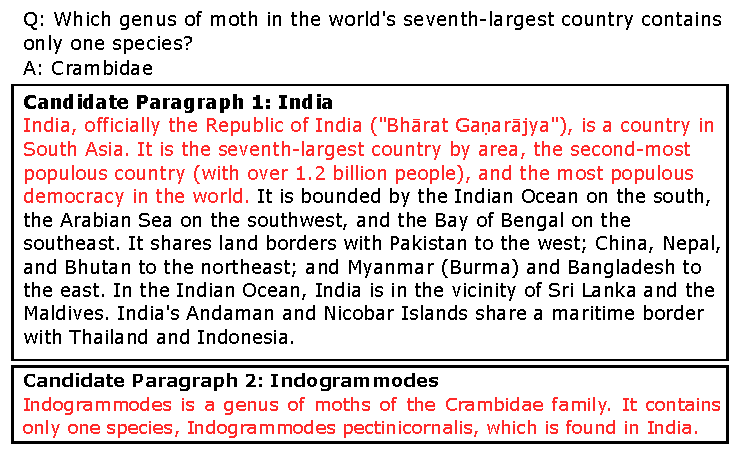
\includegraphics[width=\linewidth]{fig/fig_1_hotpot_example.pdf} % Adjust 'width' as needed
  \caption{A Sample question from the HotpotQA dataset}
  \label{fig:sample_hotpotqa} % For referencing the figure in the text
\end{figure}

%TODO: brief description of non-graph-based approaches

The first step in Graph-based approaches is to construct either an entity graph \cite{RN81} \cite{RN117} \cite{RN122} \cite{RN141} \cite{RN91} \cite{RN130} 
or a hierarchical graph \cite{RN124} \cite{RN119} \cite{RN130}, to model the relationships in the texts. Once this is done, a GNN-based 
reasoning module is used to perform multi-hop reasoning over the graph, and finally a prediction module is used to predict answers \cite{RN23}.
%TODO: expand this paragraph

Recently, there have been arguments as to whether GNNs are actually necessary for MHRC. Shao et al. (2020) \cite{RN127} argue that 
a graph structure may not be necessary with proper use of pre-trained models, and that the graph structure can be regarded as task-specific 
prior knowledge. Groenveld et al. (2020) \cite{RN126} showed that a simple BERT-based model can outperform a Graph-based model on the HotpotQA dataset,
and that supporting sentence identification in HotpotQA might not be a multi-hop problem at all. Wu et al. (2021) \cite{RN106} suggested that
the paragraph retrieval stage might be more important than the reasoning stage in MHRC, and that the reasoning stage might not be a multi-hop problem.
Similar arguments are also made by Min et al. (2019) \cite{RN150}.
%TODO: motivation for survey - is GNN necessary for MHRC?
%TODO: mention Min et al. argument about the MHRC Dataset problem

In this paper, we present a survey of various approaches that have been proposed for MHRC, with a focus on Graph-based approaches. We also try to
address the question of whether GNNs are actually necessary for MHRC. We first present a taxonomy of the various approaches, and then discuss the
core concepts of MHRC. We then present a detailed discussion of the various approaches, and finally conclude with a discussion of the open problems 
and future directions.
%TODO: contributions of survey

\section{Background}
%TODO

\section{Taxonomy}
%TODO

\section{Core Concepts}
%TODO
\subsection{An Overview of Current approaches}
For the purposes of understanding Graph based approaches, we will consider the following models:
DFGN \cite{RN122}, HGN \cite{RN119}, CogQA \cite{RN118}, Gated-RGCN \cite{RN91}, AMGN \cite{RN131} and DRN \cite{RN142}. We will also compare them with 
a couple of leading non-graph-based approaches: Beam Retriever \cite{RN105} (Current SOTA for HotpotQA Distractor Setting) and
HopRetriever \cite{RN149}.

\subsubsection{CogQA}
The CogQA framework \cite{RN118} is a two-stage framework, based on the \emph{Dual Process Theory} of human cognition \cite{RN137}.
The first stage is analogous to "System 1" or "Intuition", and is used to retrieve relavant information. The second stage is analogous to
"System 2" or "Reasoning", and is used to perform multi-hop reasoning over the retrieved information. A \emph{Cognitive graph} is constructed
using the extracted entities. System 2 then collects \emph{clues} which are used by System 1 to extract next-hop entities.
The Cognitive graph is initialized with the entities mention in the question $\mathcal{Q}$ and they are marked as \emph{frontier nodes}.

CogQA uses BERT \cite{RN153} for System 1. Input sentences to BERT are constructed by concatenating two functional parts 
$\text{Sentence A}$ and $\text{Sentence B}$.

$$
\underbrace{{[CLS]\: Question \: [SEP]\: clues[x; \mathcal{G}]\: [SEP]}}_{\text{Sentence A}} \underbrace{{Para[x]}}_{\text{Sentence B}}
$$

System 1 generates the semantic vector $sem[x; Q; clues]$, and pointer vectors 
$\boldsymbol{S}_{ans} , \boldsymbol{E}_{ans} $ and $\boldsymbol{S}_{hop} , \boldsymbol{E}_{hop} $ for answer and next hop spans respectively.

The primary function of System 2 is to update the hidden representations $\boldsymbol{X} \in \mathbb{R}^{n \times H}$ for all $n$ entities in $\mathcal{G}$.
System 2 uses a variant of GNNs \cite{RN2} to perform this task. The new hidden representations $\boldsymbol{X'}$ are updated as follows:

$$
\Delta = \sigma((AD^{-1})^T \sigma (\boldsymbol{X}W_1))
$$
$$
\boldsymbol{X'} = \sigma(\boldsymbol{X}W_2 + \Delta)
$$

System 2 also prepares $clues[x; \mathcal{G}]$ for System 1. Finally, a two layer fully connected network is used to predict the answer.
$$
answer = \underset{\text{answer node }x}{\mathrm{argmax}}  \mathcal{F}(\boldsymbol{X}[x])
$$

\subsubsection{DFGN}
Dynamically Fused Graph Network (DFGN) \cite{RN122} constructs a \emph{dynamic entity graph}, where a dynamic local entity graph is 
constructed for each question. It is comprised of 5 modules for paragraph selection, entity graph construction, encoding, fusion (for multi-hop reasoning),
and a final prediction layer.

The paragraph selection module for DFGN also uses a pretrained BERT-based model \cite{RN153} to select the most relavant paragraphs to the query $Q$ which 
are then concatenated to form the context $C$. Next, the entity graph is constructed with entities as nodes. The Stanford corenlp toolkit \cite{RN170} is used 
to extract entities from the context. Edges are added for sentence-level links, context-level links, and paragraph-level links. The query and context are 
concatenated and passed through a BERT-based model, and further through a bi-attention layer to obtain the contextualized representations.

The fusion block has 3 major steps: 1. Doc2Graph, where the text spans are converted into entity embeddings, 2. Information propogation on the entity graph and 3. Graph2Doc, where 
information passes from the entity back to the tokens. In the 2nd step, we utilize a GNN based on Graph Attention Networks \cite{RN7} to propogate node information. The prediction layer is 
similar to \cite{RN116}

\subsubsection{HGN}
Hierarchical Graph Network (HGN) \cite{RN119} proposes a hierarchical graph network with nodes for different granularity levels, like questions, paragraphs, sentences, and entities.
Large-scale pre-trained language models like BERT \cite{RN153} or RoBERTa \cite{RN171} are used to encode the input text. The encoded representations are then used to construct the hierarchical graph.
It uses a multi-task prediction module which performs multiple roles like paragraph selection, supporting fact selection, entity prediction and answer span extraction.

\subsubsection{AMGN}
Asynchronous Multi-grained Graph Network \cite{RN131} or AMGN is currently the best performing graph-based approach on the HotpotQA dataset.
The authors point out several limitations of existing GNN based approaches. Previous methods perform message-passing synchronously,
which prevents reasoning in a fine-grained logical order. Secondly, previous methods only consider the  updated entity nodes
%TODO describe previous limitations
They propose AMGN which uses an asynchronous message-passing mechanism on multi-grained nodes, which mimics the the logical order of multi-hop reasoning.
RoBERTa \cite{RN171} is used to encode the question and the context. A heterogeneous graph is constructed with nodes for sentences and entities. The algorithm
then performs asynchronous message-passing on the graph, dependent on the relationship level between the nodes (entity-entity $\to$ entity-sentence $\to$ sentence-sentence).

\subsubsection{HopRetriever}
HopRetriever \cite{RN149} is a non-graph-based approach that focuses on open-domain QA, and thus is evaluated on HotpotQA's \emph{fullwiki} setting.
Firstly, the top 500 documents are retrieved based on their TF-IDF scores with respect to the query. The supporting documents
are then iteratively retrieved and supporting sentences are predicted from the retrieved documents. Finally, the answer is extracted 
from the supporting documents using BERT.

\subsubsection{Beam Retrieval}
 Zhang et al. (2023)\cite{RN105} introduce Beam Retrieval, which is a retrieval approach that uses a beam search to retrieve the relavant paragraphs. It keeps multiple 
hypotheses in consideration at each step, and is thus suited for questions requiring variable hop reasoning. A Supervised Reader or a zero-shot LLM is used 
for the reading module. It achieves strong performance and has achieved SOTA on the HotpotQA dataset \cite{RN116}.


\subsection{Evaluating the effectiveness of Graph-based approaches}

For a long while, Graph based approaches were seen as the SOTA for MHRC. However, recently, there have been arguments as to whether GNNs are actually necessary for MHRC. The best performing models 
on the HotpotQA dataset \cite{RN116} are non-graph-based approaches \cite{RN105} \cite{RN149}. 

Min et al. (2019) \cite{RN150} argue that constructing large multi-hop datasets is difficult, and that the current datasets like HotpotQA can be solved with single-hop approaches.
They also suggest that more focus should be given to the retrieval stage, and that the reasoning stage, atleast for current datasets might not be a multi-hop problem. They noted that
humans could solve over 80\% of HotpotQA questions with one gold paragraph withheld. This indicates that current datasets may not be suitable for evaluating the effectiveness of 
graph-based approaches.

Shao et al. (2020) \cite{RN127} argue that a graph structure may not be necessary with proper use of 
pre-trained models, and that the graph structure can be regarded as task-specific prior knowledge. For their approach,
they reimplement DFGN \cite{RN122} as their baseline to perform their evaluations. They use RoBERTa \cite{RN171} to retrieve paragraphs, and to encode query and context 
A fine-tuned pre-trained BERT Model is used to extract entities from candidate paragraphs. They compare the results with the fusion block, and also by removing the fusion block and directly feeding the 
outputs of the pre-trained layer directly to the prediction layer. They find that by using a fine-tuning approach, models with and without graph fusion block can reach almost equal results.

Groenveld et al. (2020) \cite{RN126} showed that a simple BERT-based model can outperform a Graph-based model on the HotpotQA dataset.
Their results show that a simple model that identifies relavant paragraphs independent of each other performs unexpectedly well, as compared to 
jointly identifying the paragraphs through methods like graph networks. Their results indicate that HotpotQA might not be suitable to demonstrate the 
value of more complex retrieval techniques, and that supporting sentence identification in HotpotQA might not be a multi-hop problem at all.

Wu et al. (2021) \cite{RN106} models the multi-hop reasoning nature in the retrieval module rather than the reader module, avoiding the need for a graph-based reasoning module.
It highlights the limitations of graph modeling for MHRC, which requires Named Entity Recognition and also requires rigid rule-based graph construction.
They also point out that retrieval of evidence paragraphs is essentially a ranking problem rather than individual sequence classification.
They also consider the multi-hop nature of paragaph retrieval and that secondary evidence extraction is usually dependent on the previous evidence.
The Select-to-Guide (S2G) model outperfomed all graph-based models reaching new SOTA on HotpotQA.


%TODO: add a table summarizing the results of the various approaches if applicable on same dataset

\subsection{Analysis of Multi-hop Datasets}
%TODO graph based models are still pretty good in the fullwiki setting - maybe that is a potential future direction?

HotpotQA seems to be the de-facto dataset for evaluating MHRC models. However, there have been arguments that the dataset itself is flawed. 
Several studies \cite{RN176} \cite{RN175} \cite{RN154} \cite{RN150} indicate that many questions in HotpotQA can be answered using heuristics, as they 
have biases and reasoning shortcuts \cite{RN177}.



\section{Related Work}
%TODO

\section{Conclusion}
%TODO

% add bibliography
\bibliographystyle{ACM-Reference-Format}
\bibliography{bib.bib}

\end{document}
\endinput
%%
%% End of file
